\documentclass[twoside, 12pt]{book}
\linespread{1.25}

\usepackage[a4paper,top=2.5cm,bottom=2.5cm,left=3.5cm,right=2cm]{geometry}
\usepackage[utf8]{inputenc}
\usepackage{amsthm}
\usepackage[slovak]{babel}
\usepackage{graphicx}
\newtheorem{example}{Príklad}

%[]

\title{Zbierka úloh z Testovania 9\\

\includegraphics{assets/educat_logo.png}}
\date{}
\pagestyle{plain}
\usepackage[hidelinks]{hyperref}

\theoremstyle{definition}
\newtheorem{solution}{Riešenie}

\begin{document}
	\maketitle
	\tableofcontents
	
	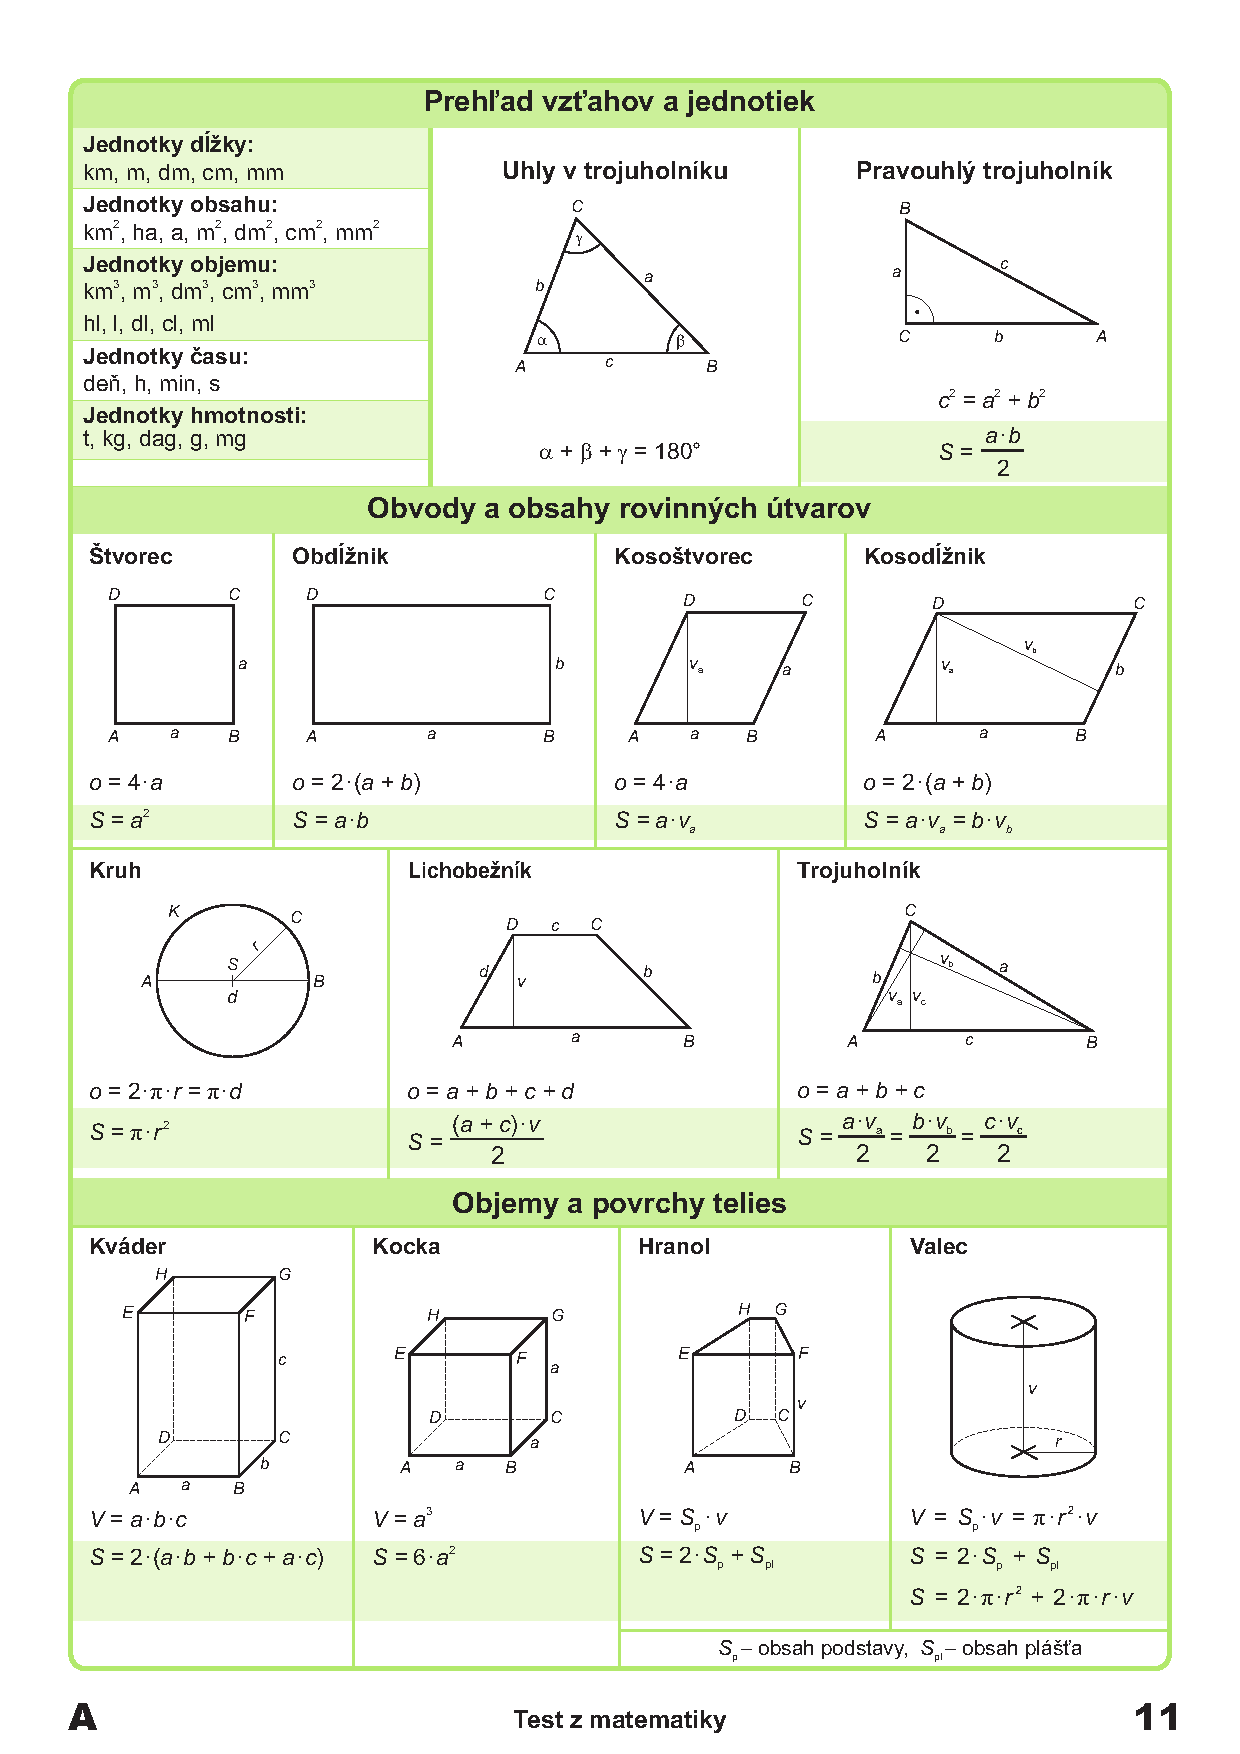
\includegraphics[width=\linewidth]{assets/vzorce.pdf}
	
	\chapter{Aritmetika a teória čísel}

\begin{example}
	Vypočítaj $1,5^2 + 1,6^2 + 1,7^2$.
\end{example}

\begin{example}
	Mesačník o zdravej výžive stojí 2,90€. Pán Milan si objednal ročné predplatné, zaplatil zaň 29,50€. Koľko eur ušetril kúpou predplatného.
\end{example}

\begin{example}
	Číselná os na obrázku je zobrazená na 8 zhodných sekov. Bod A je obrazom reálneho čísla. Uveď toto číslo ako zlomok v základnom tvare.
	\begin{center}
		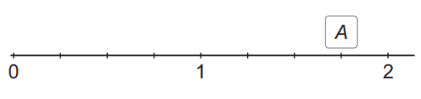
\includegraphics{assets/os1.png}
	\end{center}
\end{example}

\begin{example}
	Otec nechal synovi nasledujúci odkaz: „Ak chceš vedieť heslo na wifi, usporiadaj čísla od najmenšieho po najväčšie.“ \\
	$\frac{4}{3} = M$, $\frac{5}{4} = S$, $1,4 = P$, $1,5 = L$
	Ktoré heslo je správne?
	\begin{enumerate}
		\item LPMS
		\item MSPL
		\item PSLM
		\item SMPL
	\end{enumerate}
\end{example}

\begin{example}
	Na číselnej osi je vyznačený obraz čísla a. \\
	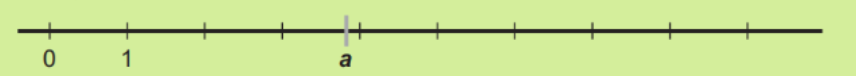
\includegraphics{assets/os2.png}\\
	Ktoré z uvedených piatich vzťahov platí pre číslo a?
	\begin{enumerate}
		\item $a - 6 > 0$
		\item $4 - a > 0$
		\item $5 - a < 0$
		\item $a - \frac{16}{3} < 0$
		\item $-1 - a < 0$
	\end{enumerate}
\end{example}

\begin{example}
	Na číselnej osi sú body A, B, C obrazmi reálnych čísel. Vypočítaj hodnotu výrazu A + B - C a výsledok zapíš v tvare desatinného čísla.\\
	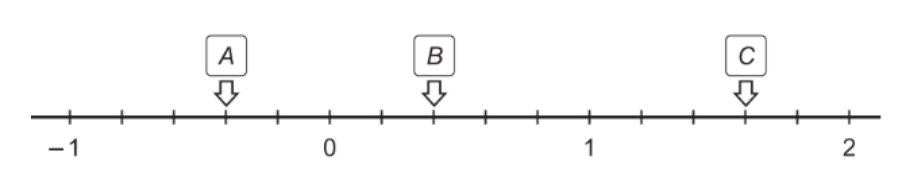
\includegraphics{assets/os3.png}
\end{example}

\begin{example}
	Na číselnej je vyznačených šedť rovnako dlhých úsekov. Bod A je obrazom reálneho čísla. Zapíš toto číslo ako zlomok v základnom tvare. \\
	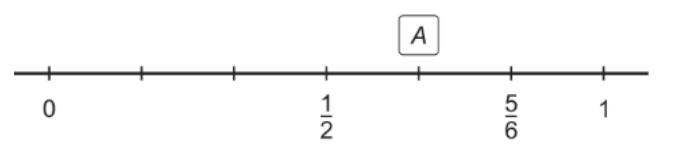
\includegraphics{assets/os4.png}
\end{example}

\begin{example}
	Desiati priatelia sa dohodli, že si objednajú pizze spolu, aby využili akciu, kde dostanú každú štvrtú pizzu zadarmo. Jedna pizza stojí 6€. Koľko eur ich vyšla 1 pizza v priemere, ak si objednali 10 pízz. Výsledok uveď s presnosťou na 2 desatinné miesta.
\end{example}

\begin{example}
	Ktorá z nasledujúcich nerovností platí? \\
	Nerovnosť 1: \fbox{$3^2 > 2^3$}. Nerovnosť 2: \fbox{$(-3)^2 < (-2)^3$}.\\
	\begin{enumerate}
		\item Platí len nerovnosť 1.
		\item Platí len nerovnosť 2.
		\item Platia obe nerovnosti.
		\item Neplatí ani jedna nerovnosť.
	\end{enumerate}
\end{example}

\begin{example}
	Číslo na nazýva dokonalé, ak je súčet jeho deliteľov okrem seba samého rovný tomuto číslu.\\
	Napríklad číslo 28 je dokonalé. Súčet jeho deliteľov 1, 2, 4, 7, 14 je 28. \\
	Ktoré z nasledujúcich čísel je tiež dokonalé?
	\begin{enumerate}
		\item 14
		\item 12
		\item 8
		\item 6
	\end{enumerate}
\end{example}

\begin{example}
	Riadky tabuľky sú označené písmenami R, S, T a stĺpce číslami 1, 2, 3. Do výrazu \textbf{R2 - S3 + T1} dosaď príslušné čísla a vypočítaj jeho hodnotu. \\
	\begin{center}
		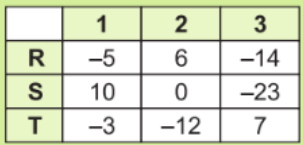
\includegraphics{assets/tab.png}
	\end{center}
	
\end{example}

\begin{example}
	Na farme chovajú 110 kusov hydiny (sliepky, morky, kačky a husi). Sliepky predstavujú polovicu. moriek je 10 a kačiek je o 7 viac ako husí. Koľko husí chovajú na farme?
\end{example}

\begin{example}
	Koľkokrát je číslo $5 \cdot 10^5$ väčšie ako číslo $125 \cdot 10^3$?
\end{example}

\begin{example}
	Vypočítaj dve tretiny z troch štvrtín. Výsledok zapíš ako zlomok v základnom tvare.
\end{example}

\begin{example}
	Traja súrodenci si objednali pizzu. Miška zjedla štvrtinu z pizze. Lenka zjedna tretinu zo zyšku a Patrik zjedol polovicu z toho, čo nechala Lenka. Zvyšok si nechali zabaliť domov. Akú časť pizze im zabalili? Výsledok zapíšte ako zlomok v základnom tvare. 
\end{example}

\begin{example}
	Pavlína má stovky svojich fotografií z dovolenky uložené na pamäťových kartách. Všetky fotografie dala vytlačiť. V tabuľke sú uvedené počty fotografií a ceny za ich vytlačenie. Koľko eur zaplatila Paulína za vytlačenie všetkých svojich fotografií s rozmermi $10 \times 15$ cm.
	
	\begin{center}
		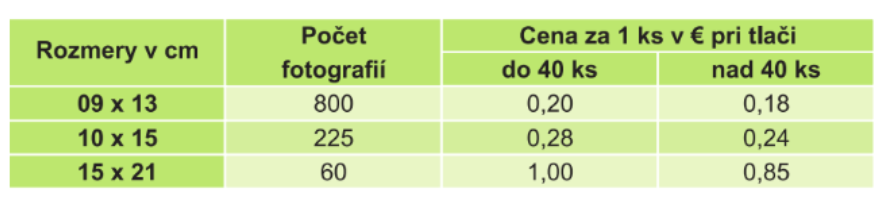
\includegraphics{assets/fotky.png}
	\end{center}
\end{example}

\begin{example}
	Vypočítaj a výsledok zapíš v tvare desatinného čísla.\\ $\frac{3}{4} -1\frac{2}{5} + 0,5$.
\end{example}

\begin{example}
	Máme číslo A = 753 672. Vypočítaj rozdiel čísla A zaokrúhľeného na stovky a čísla A zaokrúhleného na desaťtisíce.
\end{example}

\begin{example}
	Vypočítaj $\frac{1}{3} + \frac{1}{3} \cdot \frac{1}{3} + \frac{1}{3}$.\\
	\begin{enumerate}
		\item $0.\overline{8}$
		\item $0.\overline{7}$
		\item $0.\overline{5}$
		\item $0.\overline{4}$
	\end{enumerate}
\end{example}

\begin{example}
	Vyber mocninu, ktorá má najväčšiu hodnotu.
	\begin{enumerate}
		\item $5^2$
		\item $4^3$
		\item $3^4$
		\item $2^5$
	\end{enumerate}
\end{example}

\begin{example}
	Vypočítaj $800 - 700 \div 2 + 100 \cdot 14.67$.
\end{example}

\begin{example}
	Na číselnej osi sú zobrazené M, A, V. Vypočítaj M + A + V. \\
	\begin{center}
		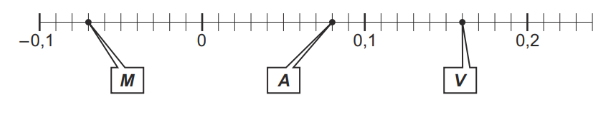
\includegraphics{assets/os5.png}
	\end{center}
\end{example}

\begin{example}
	Vypočítaj $(-0,7)^2 \cdot 10^2 + (-0,2 \cdot 10)^3$.
\end{example}

\begin{example}
	Z čísel uvedených na kartičkách sčítaj najmenjšie a najväčšie číslo.\\
	\begin{center}
		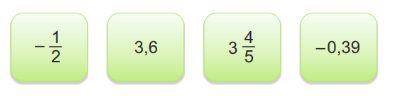
\includegraphics{assets/karticky.png}
	\end{center}
\end{example}

\begin{example}
	Pri tovare \textbf{B} bola ponuka: \textbf{Ak si zoberiete 6 kusov, zaplatíte len za 4 kusy}. Jeden kus tohoto tovaru stojí 7€. Mária si zobrala 31 kusov tohoto tovaru. Koľko eur zaplatila za tovaru?
\end{example}

\begin{example}
	Vypočítaj hodnotu výrazu $\frac{1}{4} + \frac{3}{2} - \frac{5}{6}$. Výsledok uveď ako desatinné číslo na dve desatinné miesta.
\end{example}

\begin{example}
	Vypočítaj súčin výrazov A a B. \\
	$A = 10 - (9 - 8) - (6 - 7)$\\
	$B = 4 \cdot 10^2 + 5 \cdot 10 + 9$
\end{example}

\begin{example}
	Ktoré číslo je na číslenej osi rovnako vzdialené od čísel 299 a 1051?
\end{example}

\begin{example}
	Anka si na výlet kúpila 1,5 litra minerálky. Tri pätiny z nej vypila. Vyber pravdivé tvrdenia. \\
	\begin{enumerate}
		\item Vypila menej ako polovicu.
		\item Zostalo jej 6 dl minerálky.
		\item Vypila viac ako jeden liter minerálky.
		\item Zostali jej dve tretiny minerálky.
	\end{enumerate}
\end{example}

\begin{example}
	V mise bolo 100 sliviek. Igor si z nej zobral 2 slivky a Viera si zobrala $\frac{4}{7}$ zo zvyšku. Koľko sliviek zostalo v mise?
\end{example}

\begin{example}
	Kamaráti Filip a Tibor počítali príklady z matematiky. \\
	Filip: $3 - 12 \cdot 5 -18 = -75$\\
	Tibor: $40 - (90 - 	55) \div 5 = 1$
\end{example}

\begin{example}
	Vypočítaj $\frac{1}{2} + \frac{2}{3} \cdot \frac{3}{4} - \frac{4}{5} \div \frac{6}{5}$. Výsledok uveď ako zlomok v základnom tvare.
\end{example}

\begin{example}
	Adam a Eva počítali príklady.  \\
	Adam uviedol, že výsledok príkladu $0 - (-2)^3$ je 8. \\
	Eva uviedla, že výsledok príkladu $(-3)^2 - 1$ je -8. \\
	Vyber pravdivé tvrdenie.
	\begin{enumerate}
		\item Obaja uviedli správne výsledky.
		\item Len Adam uviedol správny výsledok.
		\item Len Eva uviedla správny výsledok.
		\item Ani jeden neuviedol správny výsledok.
	\end{enumerate}
\end{example}

\begin{example}
	Dvojnásobok čísla $4^2$ odpočítaj od čísla $\sqrt{\frac{9}{16}}$. Výsledok uveď ako zlomok v základnom tvare.
\end{example}
	\chapter{Lineárne výrazy, rovnice a nerovnice}

\begin{example}
	V sčítacej pyramíde sa súčet čisel v susedných poličkách rovná číslu v políčku nad nimi. Ktoré číslo patrí v nasledujúcej sčítacej pyramíde na miesto otáznika?
	\begin{center}
		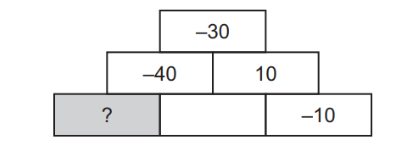
\includegraphics{assets/pyramida1.png}
	\end{center}
\end{example}

\begin{example}
	Pani Klára má v banke povolené prečerpanie účtu. Aktuálne je na jej účte mínusový zostatok -125,80 €. Po pripísaní výplaty sa suma na jej účte zmenila 721,50 €. Vypočítaj výšku výplaty pani Kláry v eurách.  
\end{example}

\begin{example}
	Jolana číta detektívku. Prečítala už 270 strán. Koľkostrán ma celá detektívka, ak Jolane zostáva prečítať $\frac{2}{5}$ detektívky.
\end{example}

\begin{example}
	Štyria súrodenci si sporia na spoločnú kolobežku. Tomáš nasporil o 30 € viac ako Eva, Roman dvakrát viac ako Eva a Soňa o 20\% viac ako Eva. Spolu už nasporili 290 €. Ktoré z nasledujúcich tvrdení je nesprávne?
	
	\begin{enumerate}
		\item Sestry nasporili menej ako ich bratia.
		\item Bratia nasporili 3-krát viac ako Soňa.
		\item Tomáš nasporil o 20 € viac ako Roman.
		\item Eva nasporila o 10 € ako Soňa.
	\end{enumerate}
\end{example}

\begin{example}
	Nájdi riešenie rovnice $6x - (2 - 2x) = 3(x-4)$.
\end{example}

\begin{example}
	Ktoré číslo nie je riešením nasledovnej nerovnice: $3 < 2(3x-9)$?
	
	\begin{enumerate}
		\item 6
		\item 5
		\item 4
		\item 3
	\end{enumerate}
\end{example}

\begin{example}
	Rieš nerovnicu $2x - 77 > 93$ a urči, koľko dvojciferných čísel je riešením tejto nerovnice.
\end{example}

\begin{example}
	Súrodenci Novákovci potrebovali odvážiť psov Birna a Astu. Psy odmietali pokojne sedieť na váhe, preto sa odbážili spolu s nimi tak, ako je znázornené na obrázkoch. Koľko kilogramov vážila Asta?
	
	\begin{center}
		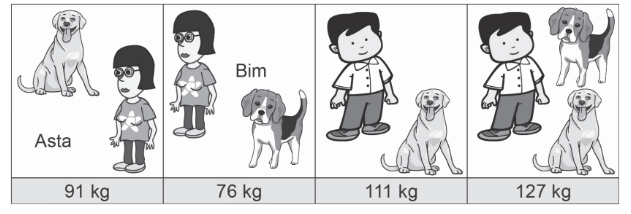
\includegraphics{assets/novakovci.png}
	\end{center}
\end{example}

\begin{example}
	Vypočítaj hodnotu výrazu $2x + 3(2 - y)$ pre $x = 3$ a $y = -1$.
\end{example}

\begin{example}
	Na ľavej strane rovnice je výraz $x - 2,4$. Zisti, ktorý z výrazov patrí na pravú stranu rovnice, aby rovnica mala koreň 2,8.
	
	\begin{enumerate}
		\item $3(x - 1,1)$
		\item $2(3 - x)$
		\item $3(x + 1,1)$
		\item $2(3 + x)$
	\end{enumerate}
\end{example}

\begin{example}
	Vyrieš rovnicu a výsledok uveď s presnosťou na stotiny: $11(x-1) = 11 - (1 + x)$.
\end{example}

\begin{example}
	Na školskom výlete x chlapcov. Dievčat bolo o 6 menej ako chlapcov. Dvojsedačkovou lanovkou sa všetci vyviezli z dolnej na hornú stanicu. Rozhodni, ktorý výraz vyjadruje počet sedačiek obsadených žiakmi, ak každá bola obsadené dvomi žiakmi.
	
	\begin{enumerate}
		\item $(x - 6) \div 2$
		\item  $(x - 6 + x - 6) \div 2$
		\item $(x + x) \div 2 - 6$
		\item $(x + x - 6) \div 2$
	\end{enumerate} 
\end{example}

\begin{example}
	Súčin troch čísel je 224. Prvé z nich je 10, druhé je 50-krát menšie ako prvé. Vypočítaj tretie číslo. 
\end{example}

\begin{example}
	Ktoré číslo treba doplniť na miesto otáznika tak, aby mala rovnica koreň 3? $2x - -3(5-x) - 1 = x - $ ?
\end{example}

\begin{example}
	Ktoré číslo má tú vlastnosť, že ak ho zväčšíme o 7, dostaneme číslo, ktoré má rovnakú absolútnu hodnotu ako toto číslo?
\end{example}

\begin{example}
	Nad každou dvojicou vedľa seba zobrazených výrazov na obrázku je ich súčet. Zistite, ktorý výraz bude na najvyššom mieste na obrázku.
	
	\begin{center}
		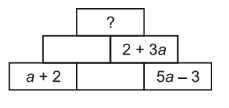
\includegraphics{assets/pyramida2.png}
	\end{center}
\end{example}

\begin{example}
	Urči číslo, ktoré je riešením rovnice $333 - 33x = 3$.
\end{example}

\begin{example}
	Tretina neznámeho čísla je rovnako veľká ako päťnásobok tohoto rozdielu tohoto neznámeho čísla a čísla 28. Urči toto neznáme číslo.
\end{example}

\begin{example}
	Môj pes je o 4,4 kg ťažší ako moja mačka. Spolu vážia 15 kg. Koľko váži môj pes?
\end{example}

\begin{example}
	Ktorý z výrazov má pre hodnotu $x = -3$ hodnotu 10?
	
	\begin{enumerate}
		\item $7 - x$
		\item $13 - x$
		\item $x - 13$
		\item $x - 7$
		
	\end{enumerate}
\end{example}

\begin{example}
	Ktoré najmenšie celé číslo je riešením nerovnice $0.5x - 7 < 2x - 50$?
\end{example}

\begin{example}
	Eugen má o 27 kníh viac ako Daniela, ale 3-krát menej ako Tomáš. Tomáš má 132 kníh. Koľko kníh má Daniela?
\end{example}

\begin{example}
	Pán Martin má v knižnici 150 kníh. Rozdelil ich do piatich kategórií. Románov je 75, encyklopédií je 5-krát menej ako románov. Detských kníh má o 4 viac ako cestopisov. V kategórii hobby si nechal 20 kníh. Koľko cestopisov má Martin vo svojej knižnici.
\end{example}

\begin{example}
	Vypočítaj hodnotu výrazu y pre = = -2 podľa nasledovnej schémy.
	
	\begin{center}
		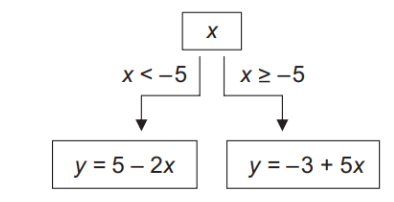
\includegraphics{assets/schema.png}
	\end{center}
\end{example}

\begin{example}
	V nasledujúcej tabuľke uvedený cenník listov kúpaliska.
	
	\begin{center}
		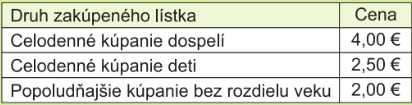
\includegraphics{assets/tab3.png}
	\end{center}
	
	Počas dňa si na kúpalisko kúpilo lístok $x$ dospelých a $y$ detí. Na popoludňajšie kúpanie sa predalo 17 lístkov. Ktorý výraz vyjadruje tržbu kúpaliska počas celého dňa?
	
	\begin{enumerate}
		\item $6,5xy + 17$
		\item $4x + 2,5y + 17$
		\item $4x + 2,5y + 34$
		\item $6,5xy + 34$
	\end{enumerate}
\end{example}
	\chapter{Priama a nepriama úmernosť, pomer, percentá a promile}


\section{Priama úmernosť}

\section{Neprieme úmernosť}

\section{Pomer}

\section{Percentá a promile}
	\chapter{Geometria}

\section{Planimetria}

\subsection{Uhly}

\subsection{Rovinné útvary}

\subsection{Goniometria a trigonometria}

\section{Stereometria}
	\chapter{Kombinatorika, pravdepodobnosť a štatistika}
\label{chap:pas}

\section{Kombinatorika}

\subsection{Faktoiál a permutácie}

\subsection{Variáce bez opakovania}

\subsection{Variáce s opakovaním}

\subsection{Kombinácie}

\subsection{Pravidlo súčtu a súčinu}

\newpage

\section{Pravdepodobnosť}

\subsection{Kombinatorická pravdepodobnosť}

\subsection{Geometrická pravdepodobnosť}

\newpage

\section{Štatistika}
	\chapter{Výsledky}

\begin{solution}
	$7.7$
\end{solution}
	
\end{document}